% This file was converted to LaTeX by Writer2LaTeX ver. 1.6.1
% see http://writer2latex.sourceforge.net for more info
\documentclass[a4paper]{article}
\usepackage[utf8]{inputenc}
\usepackage{amsmath}
\usepackage{amssymb,amsfonts,textcomp}
\usepackage[T1]{fontenc}
\usepackage[english]{babel}
\usepackage{color}
\usepackage[top=2.499cm,bottom=2cm,left=2cm,right=2cm,nohead,nofoot]{geometry}
\usepackage{array}
\usepackage{supertabular}
\usepackage{hhline}
\usepackage{hyperref}
\hypersetup{colorlinks=true, linkcolor=blue, citecolor=blue, filecolor=blue, urlcolor=blue}
\usepackage{graphicx}
\providecommand\textsubscript[1]{\ensuremath{{}_{\text{#1}}}}
\makeatletter
\newcommand\arraybslash{\let\\\@arraycr}
\makeatother
% Footnote rule
\setlength{\skip\footins}{0.119cm}
\renewcommand\footnoterule{\vspace*{-0.018cm}\setlength\leftskip{0pt}\setlength\rightskip{0pt plus 1fil}\noindent\textcolor{black}{\rule{0.25\columnwidth}{0.018cm}}\vspace*{0.101cm}}
\setlength\tabcolsep{1mm}
\renewcommand\arraystretch{1.3}
\title{}
\author{}
\date{2021-03-17}
\begin{document}
\title{Optimal control strategies to prevent the hospital beds collapse during Covid-19 outbreak}
\maketitle

{\centering
\textit{Leonardo Pio Lo Porto}
\par}

{\centering
\textit{Simone Rotondi }
\par}


\bigskip

\textbf{\textcolor[rgb]{0.07450981,0.078431375,0.07450981}{Abstract: }}In 2020 the world has faced a serious challenge
since the breakout of corona-virus started in Wuhan, China. The deathly disease has killed about 1.770.000 and infected
more than 80 millions humans around the globe since December 2019 to 27 of December 2020. 

The paper presents a new mathematical model for the SARS-CoV-2 virus propagation, designed to include all the possible
actions to prevent the spread and to help in the healing of infected people, including the new inoculation to the
SARS-CoV-2. The objective of this project is to propose the possibility of optimal controls over the susceptible and
the infected subjects considering different cost functions in order to see the effects of different optimised control
actions on the evolution of the epidemic spread and in particular how these controls should be tuned in order to avoid
the hospital beds collapse. \textcolor[rgb]{0.07450981,0.078431375,0.07450981}{The optimal control analysis was carried
out using the Pontryagin’s maximum principle to figure out the optimal strategy necessary to curtail the disease.}and
the existence of the optimal solution is assessed. Numerical evaluations are developed for a more intuitive and
immediate presentation, showing the consequences on the classes of interest. 


\bigskip

\setcounter{tocdepth}{6}
\renewcommand\contentsname{Indices}
\tableofcontents

\bigskip


\bigskip


\bigskip


\bigskip

\section{1. Introduction}
\hypertarget{Toc66707022}{}\textcolor[rgb]{0.07450981,0.078431375,0.07450981}{Coronavirus disease 2019 (COVID-19) is a
disease caused by severe acute respiratory syndrome coronavirus 2 (SARS CoV-2). \ }

\textcolor[rgb]{0.07450981,0.078431375,0.07450981}{Italy has been severely affected[5]. After the first indigenous case
on 21 February 2020 in Lodi province, several suspect cases (initially epidemiologically linked) began to emerge in the
south and southwest territory of Lombardy[6]. A ‘red zone’, encompassing 11 municipalities where SARS-CoV-2 infection
was endemic, was instituted on 22 February 2020, and put on lockdown to contain the emerging threat. A campaign to
identify and screen all close contacts with confirmed cases of COVID-19 resulted in taking 691,461 nasal swabs as of 5
April 2020. Of the 128,948 detected cases, 91,246 were currently infected (28,949 hospitalized, 3,977 admitted to
intensive care units (ICUs) and 58,320 quarantined at home), 21,815 had been discharged due to recovery and 15,887 had
died7. In the early days of the epidemic in Italy, both symptomatic and asymptomatic people underwent screening. A
government regulation dated 26 February 2020 limited screening to symptomatic subjects only[8]. On 8 March 2020, to
further contain the spread of SARS-CoV-2, the red zone was extended to the entire area of Lombardy and 14 more northern
Italian provinces. On 9 March 2020, lockdown was declared for the}

\textcolor[rgb]{0.07450981,0.078431375,0.07450981}{entire country[9] and progressively stricter restrictions were
adopted. COVID-19 displays peculiar epidemiological traits when compared with previous coronavirus outbreaks of
SARS-CoV and }\textcolor[rgb]{0.07450981,0.078431375,0.07450981}{MERS-CoV. According to Chinese data[10], a large
number of transmissions, both in nosocomial and community settings, occurred through human-to-human contact with
individuals showing no or mild symptoms. The estimated basic reproduction number
(}\textit{\textcolor[rgb]{0.07450981,0.078431375,0.07450981}{R}}\textcolor[rgb]{0.07450981,0.078431375,0.07450981}{0)
for}

\textcolor[rgb]{0.07450981,0.078431375,0.07450981}{SARS-CoV-2 ranges from 2.0 to 3.5[11–13], which seems comparable, or
possibly higher, than for SARS-CoV and MERS-CoV. High viral loads of SARS-CoV-2 were found in upper respiratory
specimens of patients showing little or no symptoms, with a viral shedding pattern akin to that of influenza
viruses[14]. Hence, inapparent transmission may play a major and underestimated role in sustaining the outbreak.}

\textcolor[rgb]{0.07450981,0.078431375,0.07450981}{Until the end of December the disease had neither approved medicine
nor vaccine and has made governments and scholars search for drastic measures in combating the pandemic. The 26th of
}\textbf{\textcolor[rgb]{0.07450981,0.078431375,0.07450981}{December the first 10.000 doses of vaccine have been
delivered in Italy but the effectiveness of it is not yet guaranteed and the first side effects have been occured in
different countries.}}

\textcolor[rgb]{0.07450981,0.078431375,0.07450981}{Predictive mathematical models for epidemics [15–18] are fundamental
to understand the course of the epidemic and to plan effective control strategies. One commonly used model is the SIR
model[19] for human-to-human transmission, which describes the flow of individuals through three mutually exclusive
stages of infection: susceptible, infected and recovered. More complex models can accurately portray the dynamic spread
of specific epidemics. For the COVID-19 pandemic, several models have been developed for specific classes of
infections, to better describe their propagation and to particularize the specific control actions against its spread.}

\textcolor[rgb]{0.07450981,0.078431375,0.07450981}{In this paper a quite rich model is proposed, composed by 8 different
classes and the model parameters are identified on the basis of the available data. To have a more detailed model all
the known preventive and active actions that can be put in place are considered, at an organizational and decisional
level as well as from a medical point of view, to contain the virus spread. For the aim of our work, the model explains
in a better way the compartments of infected people drawing a distinction between different type of infectious and
paying attention to those that are in the hospitals. }

\textcolor[rgb]{0.07450981,0.078431375,0.07450981}{Regrettably, the spread of the virus and mortality due to COVID-19
has continued to increase daily. }\textbf{\textcolor[rgb]{0.07450981,0.078431375,0.07450981}{Hence, it is imperative to
control the spread of the disease particularly using nonpharmacological strategies (and in a second case
pharmacological one) such as quarantine, isolation, and public health education.}}

\textcolor[rgb]{0.07450981,0.078431375,0.07450981}{This work studied the effect of these different control strategies
using mathematical modeling and optimal control approach to ascertain their contributions in the dynamic transmission
of COVID-19. }

\textcolor[rgb]{0.07450981,0.078431375,0.07450981}{In the following paragraph the model is presented and described. }


\bigskip

\section{2. Methods}
\hypertarget{Toc66707023}{}\subsection{2.1 Mathematical Model }
\hypertarget{Toc66707024}{}\textcolor[rgb]{0.07450981,0.078431375,0.07450981}{The mathematical model here adopted is an
enrichment of a classical SEQIR one, usually adopted to describe the dynamic of epidemic spreads in presence of a virus
incubation phase (E) in which the quarantine compartment (Q) is considered. To the standard SEQIR model more classes
are added, the possible ways of intervention are modelled in order to make available some numerical evaluations about
the potential epidemic diffusion depending on the different strategies. We have considered the
}\textit{\textcolor[rgb]{0.07450981,0.078431375,0.07450981}{SEI}}\textit{\textcolor[rgb]{0.07450981,0.078431375,0.07450981}{\textsubscript{a}}}\textit{\textcolor[rgb]{0.07450981,0.078431375,0.07450981}{QI}}\textit{\textcolor[rgb]{0.07450981,0.078431375,0.07450981}{\textsubscript{1}}}\textit{\textcolor[rgb]{0.07450981,0.078431375,0.07450981}{I}}\textit{\textcolor[rgb]{0.07450981,0.078431375,0.07450981}{\textsubscript{2}}}\textit{\textcolor[rgb]{0.07450981,0.078431375,0.07450981}{RV
}}\textcolor[rgb]{0.07450981,0.078431375,0.07450981}{epidemic model for Covid-19
transmission}\textit{\textcolor[rgb]{0.07450981,0.078431375,0.07450981}{,
}}\textcolor[rgb]{0.07450981,0.078431375,0.07450981}{where each class is defined as follow:}

\begin{itemize}
\item \textcolor[rgb]{0.07450981,0.078431375,0.07450981}{Susceptible (S): people who are not yet infected but they are
potentially plagued by the virus.}
\item \textcolor[rgb]{0.07450981,0.078431375,0.07450981}{Expose (E): people who have been infected but they still can
not spread the virus because of the incubation period. }
\item \textcolor[rgb]{0.07450981,0.078431375,0.07450981}{Infected undetected
(I\-}\textcolor[rgb]{0.07450981,0.078431375,0.07450981}{\textsubscript{a}}\textcolor[rgb]{0.07450981,0.078431375,0.07450981}{):
fraction of population that can infect the susceptible class because they are not yet detected and so they could have
contacts with susceptible people.}
\item \textcolor[rgb]{0.07450981,0.078431375,0.07450981}{Quarantined (Q): \ fraction of population detected with or
without symptoms quarantined and due to this fact they can not have contact with susceptible.}
\item \textcolor[rgb]{0.07450981,0.078431375,0.07450981}{Hospitalized infected non-ICu
(I\-}\textcolor[rgb]{0.07450981,0.078431375,0.07450981}{\textsubscript{1}}\textcolor[rgb]{0.07450981,0.078431375,0.07450981}{):
fraction of population detected, with symptoms and }\textcolor[rgb]{0.07450981,0.078431375,0.07450981}{hospitalized not
in Intensive Care (IC).}
\item \textcolor[rgb]{0.07450981,0.078431375,0.07450981}{Hospitalized infected in ICu
(I\-}\textcolor[rgb]{0.07450981,0.078431375,0.07450981}{\textsubscript{2}}\textcolor[rgb]{0.07450981,0.078431375,0.07450981}{):
fraction of population detected that due to the heavy symptoms has been hospitalized in Intensive Care (IC).}
\item \textcolor[rgb]{0.07450981,0.078431375,0.07450981}{Recovered (R): fraction of population healed from the virus and
temporarily immune.}
\item \textcolor[rgb]{0.07450981,0.078431375,0.07450981}{Vaccinated (V): fraction of population vaccinated and immune.}
\end{itemize}
\textcolor[rgb]{0.07450981,0.078431375,0.07450981}{The mathematical model proposed is the following
one\footnotemark{}:}\footnotetext{\ Note that for a better view of the system we have omitted the time dependences of
the state variables and parameters in the system that are intrinsically in.}



\bigskip

\begin{equation*}
\dot S=b-\mathit{dS}-\mathit{\beta S}I_a\left(1-u_p\right)+\mathit{\eta R}-u_{\mathit{va}}S
\end{equation*}
\begin{equation*}
\dot E=-\mathit{dE}+\mathit{\beta S}I_a\left(1-u_p\right)-\mathit{kE}
\end{equation*}
 $\dot I_a=-\mathit{dI}+\mathit{kE}-\mathit{\lambda \tau }I_a$\textcolor[rgb]{0.07450981,0.078431375,0.07450981}{\ }
$-\gamma _1I_a$

 $\dot Q=-\mathit{dQ}+\mathit{p\lambda \tau }I_a-\gamma _2Q-$\textcolor[rgb]{0.07450981,0.078431375,0.07450981}{\ }
$\sigma _1Q$\ \ \ \ \ \ \ \ \ \ \ \ \ \ \ \  \ \textit{(1)}

\begin{equation*}
\dot I_1=-dI_1+\sigma _1Q-\gamma _3I_1-\rho _1u_1I_1-\sigma _2\left(1-u_1\right)I_1+\left(1-p\right)\mathit{\lambda \tau
}I_a
\end{equation*}
\begin{equation*}
\dot I_2=-dI_2-mI_2+\sigma _2\left(1-u_1\right)I_1-\rho _2I_2u_2
\end{equation*}
\begin{equation*}
\dot R=-\mathit{dR}-\mathit{\eta R}+\gamma _1I_a+\gamma _2Q+\gamma _3I_1+\rho _1u_1I_1+\rho _2u_2I_2
\end{equation*}
\begin{equation*}
\dot V=-\mathit{dV}+u_{\mathit{va}}S
\end{equation*}
\textcolor[rgb]{0.07450981,0.078431375,0.07450981}{With initial conditions: }


$S\left(0\right)=S_0,E\left(0\right)=E_0,I_a\left(0\right)=I_a^0,Q\left(0\right)=Q_0,I_1\left(0\right)=I_1^0,I_2\left(0\right)=I_2^0,R\left(0\right)=R_0,V\left(0\right)=V_0$\textcolor[rgb]{0.07450981,0.078431375,0.07450981}{\ \ }\textit{\textcolor[rgb]{0.07450981,0.078431375,0.07450981}{(2)}}

\textcolor[rgb]{0.07450981,0.078431375,0.07450981}{And with the control bounds:}


$u_{\mathit{min}}^p{\leq}u^p\left(t\right){\leq}u_{\mathit{max}}^p,$\textcolor[rgb]{0.07450981,0.078431375,0.07450981}{\ \ \ \ \ \ \ \ }\textit{\textcolor[rgb]{0.07450981,0.078431375,0.07450981}{(3a)}}


$u_{\mathit{min}}^1{\leq}u^1\left(t\right){\leq}u_{\mathit{max}}^1,$\textcolor[rgb]{0.07450981,0.078431375,0.07450981}{\ \ \ \ \ \ \ \ }\textit{\textcolor[rgb]{0.07450981,0.078431375,0.07450981}{(3b)}}


$u_{\mathit{min}}^2{\leq}u^2\left(t\right){\leq}u_{\mathit{max}}^2,$\textcolor[rgb]{0.07450981,0.078431375,0.07450981}{\ \ \ \ \ \ \ \ (}\textit{\textcolor[rgb]{0.07450981,0.078431375,0.07450981}{3c)}}


$u_{\mathit{min}}^{\mathit{va}}{\leq}u^{\mathit{va}}\left(t\right){\leq}u_{\mathit{max}}^{\mathit{va}}$\textcolor[rgb]{0.07450981,0.078431375,0.07450981}{\ \ \ \ \ \ \ \ }\textit{\textcolor[rgb]{0.07450981,0.078431375,0.07450981}{(3d)}}

\textbf{\textcolor{red}{Where }} $u_{\mathit{min}}=0,u_{\mathit{max}}=0.9$\textbf{\textcolor{red}{\ (depending on the
type of the control we are considering the upper }}\textbf{\textcolor{red}{bound changes).}}


\bigskip


\bigskip

\textcolor[rgb]{0.07450981,0.078431375,0.07450981}{The model in Equation (1) subdivides human population into eight
mutually exclusive compartments defined previously. The uppercase letters are the state variables and they represent
the fraction of population in each stage; the considered parameters, denoted by lowercase Greek and Latin letters, are
positive numbers. The interactions among different stages of infection are visually represented in the block diagram in
Fig.1. Now we will describe the variation of each compartment to understand how the different terms flow through the
system and how the different compartments interact among them:}

\begin{enumerate}
\item \textit{\textcolor[rgb]{0.07450981,0.078431375,0.07450981}{Modelling of susceptible population (}} $\dot
S\left(t\right)$\textit{): }By the number of births per day in Italy \textit{b }and by the fraction of population that
was recovered but no longer immune by the virus ( $\mathit{\eta R}$)\textit{, }the susceptible population is augmented.
The susceptible population decreases through natural death ( $\mathit{dS}$), the interaction between a susceptible
individual and infected but not detected by testing individual ( $\mathit{\beta S}I_a$); the latter term is mitigated
by a preventive control ): it means that if the control effort in prevention, such as correctly using the mask in a
public place or during interaction with people, washing hands accurately, is strongly applied the fraction of
population infected during a contact is quite lower. Thanks to the vaccine campaign that in the last few months are
carried on by the government this compartment could decrease also thanks the vaccine control ( $u_{\mathit{va}}$). 
\item \textit{Modelling of Infected but not contagious due to the incubation period (} $\dot E\left(t\right)$\textit{):
}the fraction of population in this compartment increases due to the contact between a susceptible and an infected but
not yet detected induvial influenced by the preventive control ( $\mathit{\beta S}I_a\left(1-u_p\right)$). In this
compartment, people cannot infect a susceptible individual because of the incubation period \  $k$\ (period in which
people are infected but not ye infectious). After this period, exposed individuals flow out ( $\mathit{kE}$ ) and they
are led in the next compartment  $I_a$.
\item \textit{Modelling of Infected but not detected by testing population (} $\dot I_a\left(t\right)$\textit{): }The
income population comes from the previous compartment (E) at the end of the incubation period ( $\mathit{kE}$. Now,
those individuals are infected and infectious but not detected; they can decrease either through the natural death or
due to detection at a rate  $\lambda $ \ after a time  $\tau $ \ that represents the inverse of the mean time to swab (
$\mathit{\lambda \tau }I_a$) or, moreover, thanks to a spontaneous recovery rate  $\gamma _1$. 
\item \textit{Modelling of quarantine population (} $\dot Q\left(t\right)$\textit{): }on one hand the growth of
quarantine population depends on the detected individuals that are subjected by a parameter \textit{p }that represents
the percentage of detected people solitary confinement ( $\mathit{p\lambda \tau }I_a$). On the other hand, its
decreasing is affected by the natural death ( $\mathit{dQ}$), an healing factor that is the spontaneous recovery rate (
$\gamma _2Q$)and the complication of the disease that brings those people in hospital ( $\sigma _1Q$). 
\item \textit{Modelling of symptomatic hospitalized Infected but not in Intensive Care population (} $\dot
I_1\left(t\right)$\textit{): }in this compartment two different terms converge: one from the quarantine compartment due
to disease complications, the other comes from the remaining part of detected people ( $\left(1-p\right)\mathit{\lambda
\tau }I_a$). The reasons that are the causes of a decreasing evolution are pointed out by the following reasons:
natural death ( $dI_1$), disease complication that bring the individuals from this compartment to the infected in
intensive care class ( $\sigma _2\left(1-u_1\right)I_1$) affected by the hospital treatments (the more is the effort
the lower is the fraction of hospitalized population that flows in intensive care), spontaneous recovery ( $\gamma
_3I_1$) and “controlled” recovery thanks to the drugs and the medical staff looks after the patients ( $\rho _1u_1I_1$)
depending on the effectiveness of the control  $\rho _1$. 
\item \textit{Modelling of symptomatic hospitalized Infected in Intensive Care population (} $\dot
I_2\left(t\right)$\textit{): }this compartment is nurtured by those people that because of a complication of the
diseases are obliged to go in IC ( $\sigma _2\left(1-u_1\right)I_1$). In this compartment the only way to be recovered
( $\rho _2I_2u_2$) is using ventilator, oxygen, specific equipment and machineries that are translated in a control
parameter  $u_2$ \ and it is affected by its effectiveness  $\rho _2$. Otherwise, natural death ( $dI_2$) and death due
to the disease ( $mI_2$) are the causes of the decreasing. 
\item \textit{Modelling of recovered population (} $\dot R\left(t\right)$\textit{): }infected not yet detected,
quarantined individuals, hospitalized infected not in IC recover spontaneously from the disease ( $\gamma _1I_a+\gamma
_2Q+\gamma _3I_1$ at rates  $\gamma _1,\gamma _2,\gamma _3$ \ respectively. For hospitalized infected not in IC and in
IC it is possible to recover through a control action  $u_1$,  $u_2$ \ respectively and they are represented by the
terms  $\rho _1u_1I_1,\rho _2u_2I_2$\ (with effectiveness of the two controls  $\rho _1$,  $\rho _2$).
\item \textit{Modelling of vaccinated population (} $\dot V\left(t\right)$\textit{): }the inflow and outflow of this
compartment depend on the vaccinated fraction of susceptible population ( $u_{\mathit{va}}S$) through a control action 
$u_{\mathit{va}}$ \ representing the investment cost on vaccine and the natural death respectively ( $\mathit{dV}$).
\end{enumerate}

\bigskip

\textbf{\textcolor[rgb]{0.07450981,0.078431375,0.07450981}{Figure 1: The model.
}}\textcolor[rgb]{0.07450981,0.078431375,0.07450981}{Graphical scheme representing the interactions among different
stages of infection in the mathematical model
}\textit{\textcolor[rgb]{0.07450981,0.078431375,0.07450981}{SEI}}\textit{\textcolor[rgb]{0.07450981,0.078431375,0.07450981}{\textsubscript{a}}}\textit{\textcolor[rgb]{0.07450981,0.078431375,0.07450981}{QI}}\textit{\textcolor[rgb]{0.07450981,0.078431375,0.07450981}{\textsubscript{1}}}\textit{\textcolor[rgb]{0.07450981,0.078431375,0.07450981}{I}}\textit{\textcolor[rgb]{0.07450981,0.078431375,0.07450981}{\textsubscript{2}}}\textit{\textcolor[rgb]{0.07450981,0.078431375,0.07450981}{RV.
}}\textcolor[rgb]{0.07450981,0.078431375,0.07450981}{Each stage has a natural death rate(d) output}

[Warning: Draw object ignored][Warning: Draw object ignored][Warning: Draw object ignored][Warning: Draw object
ignored][Warning: Draw object ignored][Warning: Draw object ignored][Warning: Draw object ignored][Warning: Draw object
ignored][Warning: Draw object ignored][Warning: Draw object ignored][Warning: Draw object ignored][Warning: Draw object
ignored][Warning: Draw object ignored][Warning: Draw object ignored][Warning: Draw object ignored][Warning: Draw object
ignored][Warning: Draw object ignored][Warning: Draw object ignored][Warning: Draw object ignored][Warning: Draw object
ignored][Warning: Draw object ignored][Warning: Draw object ignored][Warning: Draw object ignored][Warning: Draw object
ignored][Warning: Draw object ignored][Warning: Draw object ignored][Warning: Draw object ignored][Warning: Draw object
ignored][Warning: Draw object ignored][Warning: Draw object ignored][Warning: Draw object ignored][Warning: Draw object
ignored][Warning: Draw object ignored][Warning: Draw object ignored]


\bigskip


\bigskip


\bigskip


\bigskip


\bigskip


\bigskip


\bigskip


\bigskip


\bigskip


\bigskip


\bigskip


\bigskip


\bigskip


\bigskip


\bigskip


\bigskip


\bigskip


\bigskip


\bigskip

The parameters of the considered model are presented in \textbf{Table 1.}

\textit{Discussion on modelling choices: }In the model, we omit the control referring to the swabs considering just the
percentage of the positive people. This choice is given by the fact that we are interested in the study of the infected
people, so we assume that all the people that are infected not yet detected are positive with a precise percentage
given by estimations on real data. 

In the model, we have decided to consider a parameter  $\rho $ \ that has the purpose to mitigate the effectiveness of
the control in the case in which the control effort is maximum. In a matter of fact, we have supposed that, even if the
effort on hospitalised control with respect to non IC units and IC units, is maximum, it is not certain that the
outcome of this choice has its maximum effectiveness. About the recoveries we have assumed that it is possible to heal
even without drugs only if the infected people are not yet detected and without symptoms (it means in
I\textsubscript{a}), quarantined (in Q) or hospitalized but not in IC. In the latter case we have considered those
infected people that go to the hospital just for a check or would have recovered also without any treatments. \ On the
other side, to be more realistic, the infected people in IC can be healed just through treatments and the usage of
ventilator and oxygen, so in this class the only way to be recovered is with a control effort. 


\bigskip


\bigskip

\textbf{\textcolor[rgb]{0.07450981,0.078431375,0.07450981}{Table 1:
}}\textcolor[rgb]{0.07450981,0.078431375,0.07450981}{parameters of the considered model}

\begin{flushleft}
\tablefirsthead{}
\tablehead{}
\tabletail{}
\tablelasttail{}
\begin{supertabular}{|m{2.391cm}m{14.209001cm}|}
\hline
\textbf{Symbol} &
\centering\arraybslash \textbf{Interpretation}\\\hline
\multicolumn{1}{|m{2.391cm}|}{\centering  $u_p$} &
{\bfseries Prior control (social distancing, masks, information campaigns)}\\\hline
\centering  $u_1$ &
{\bfseries Hospital treatments control over non-IC patients (availability of beds, medical staff, use of drugs)}\\\hline
\multicolumn{1}{|m{2.391cm}|}{{\centering  $u_2$\par}
~
} &
{\bfseries Hospital treatments control over IC patients (availability of beds in IC units, ventilator, oxygen, medial
staff)}\\\hline
\centering  $u_{\mathit{va}}$ &
{\bfseries Control over vaccine inoculation and production.}\\\hline
\multicolumn{1}{|m{2.391cm}|}{\centering  $b$} &
{\bfseries Number of births.}\\\hline
\centering  $d$ &
{\bfseries Death rate in Italy}\\\hline
\multicolumn{1}{|m{2.391cm}|}{\centering  $\beta $} &
{\bfseries Contact rate}\\\hline
\centering  $k$ &
{\bfseries Incubation period}\\\hline
\multicolumn{1}{|m{2.391cm}|}{\centering  $\lambda $} &
{\bfseries Percentage of positive}\\\hline
\centering  $p$ &
{\bfseries Percentage of quarantined people. \textit{(1-p): }percentage of hospitalized patients not in IC}\\\hline
\multicolumn{1}{|m{2.391cm}|}{\centering  $\sigma _1$} &
{\bfseries Percentage of people that from quarantine move to Covid units after complications.}\\\hline
\centering  $\sigma _2$ &
{\bfseries Percentage of people that from Covid units move to IC units after complications. }\\\hline
\multicolumn{1}{|m{2.391cm}|}{\centering  $\gamma _i$} &
{\bfseries Recovery rate without use of drugs in I\textsubscript{a}(\textit{i=1}), Q (\textit{i}=2), I\textsubscript{1}
(\textit{i}=3)}\\\hline
\centering  $m$ &
{\bfseries Death rate}\\\hline
\multicolumn{1}{|m{2.391cm}|}{\centering  $\rho _j$} &
\textbf{Control effectiveness (} $\rho _1$\textbf{\textit{ with respect to
u}}\textbf{\textit{\textsubscript{1}}}\textbf{\textit{ and }} $\rho _2$ \textbf{\textit{\ with respect to
u}}\textbf{\textit{\textsubscript{2}}}\textbf{\textit{)}}\\\hline
\centering  $\tau $ &
{\bfseries Inverse of the mean time to swab (both referring to the onset of symptoms and the time spent to know about
the contact with a positive person)}\\\hline
\multicolumn{1}{|m{2.391cm}|}{\centering  $\eta $} &
{\bfseries Inverse of the mean time to be again susceptible }\\\hline
\end{supertabular}
\end{flushleft}

\bigskip


\bigskip


\bigskip


\bigskip


\bigskip


\bigskip


\bigskip

\subsection[2.2 Model Fitting]{2.2 Model Fitting}
\hypertarget{Toc66707025}{}\textit{\textcolor{black}{2.2.1 Motivations }}

\textcolor[rgb]{0.07450981,0.078431375,0.07450981}{In this subsection we briefly discuss the main reasons
}\textcolor{red}{on why }\textcolor{black}{before the optimal control we have decided to fit some parameters of the
model. }

\textcolor[rgb]{0.07450981,0.078431375,0.07450981}{Before we could get to the optimization of the model the fitting
problem was considered. The aim of this additional step before optimization is to check that the proposed model should
follow the real data. To accomplish this task, we have had to find the parameters that would reproduce the real
behaviour. Some of those parameters was inferred based on the official data and statistics (source:
}\textcolor[rgb]{0.07450981,0.078431375,0.07450981}{Protezione Civile, Ministero della Salute, Istat) like death rate
(} $d$\textcolor[rgb]{0.07450981,0.078431375,0.07450981}{,} $m$\textcolor[rgb]{0.07450981,0.078431375,0.07450981}{),
number of births (} $b$\textcolor[rgb]{0.07450981,0.078431375,0.07450981}{), the delays } $\tau
$\textcolor[rgb]{0.07450981,0.078431375,0.07450981}{,} $\eta $\textcolor[rgb]{0.07450981,0.078431375,0.07450981}{; the
remaining ones (} $p,\gamma _i,\lambda ,\sigma _i,\rho _i$\textcolor[rgb]{0.07450981,0.078431375,0.07450981}{ plus the
base control applied by the government }
$u_{\mathit{va}},u_1,u_2,u_p$\textcolor[rgb]{0.07450981,0.078431375,0.07450981}{) has been estimated due to the lack of
information and the uncertainties on the data. (}\textbf{\textcolor[rgb]{0.07450981,0.078431375,0.07450981}{All these
parameters are bounded between 0 and 1. DA INSERIRE IN RESULTS AND DISCUSSIONS (Risposta: sono bounded by
construction)}}\textcolor[rgb]{0.07450981,0.078431375,0.07450981}{)}

\textcolor[rgb]{0.07450981,0.078431375,0.07450981}{The fitting has been performed to start the control optimization from
a more solid and realistic base so that the data source could be more easily visualized and compared.
}\textbf{\textcolor[rgb]{0.07450981,0.078431375,0.07450981}{(}}\textbf{\textcolor{black}{una stima di alcuni parametri,
secondo noi, avrebbe permesso una successiva ottimizzazione partendo da guess quanto più reali possibili e ottimizzando
i parametri in direzioni accettabili e coerenti con l’andamento)}}


\bigskip


\bigskip


\bigskip


\bigskip

\textcolor{black}{\ \ }\textit{\textcolor{black}{2.2.1 Fitting strategy and objective function definition }}

\textcolor[rgb]{0.07450981,0.078431375,0.07450981}{We have decided to fit the parameters based on data given by italian
“Protezione Civile”}\textcolor[rgb]{0.07450981,0.078431375,0.07450981}{\textsuperscript{[6]
\ }}\textcolor[rgb]{0.07450981,0.078431375,0.07450981}{on the Hospedalized non IC, Hospedalized IC, and Quarantined
people because we are mostly interested to follow in as accurate as possible way the behaviour of those individuals
that are hospitalized in Intensive Care and not due to our initial optimal control purpose. }

\textcolor[rgb]{0.07450981,0.078431375,0.07450981}{To achieve this objective the fitting strategy was to reduce the
error between the real behaviour and the estimated one by minimizing the difference between real } $Q,I_1,I_2$ \ and
\textcolor[rgb]{0.07450981,0.078431375,0.07450981}{our model. This objective can be translated in a mathematical way as
a cost function of this type:}


\bigskip


\bigskip

\begin{equation*}
J\left(r,x\right)=\int
_{t_i}^{t_f}\left(r\left(t\right)-x\left(t\right)\right)^TM\left(r\left(t\right)-x\left(t\right)\right)\mathit{dt}
\end{equation*}
\begin{equation*}
\int
_{t_i}^{t_f}\left(\left(Q_r-Q_e\right)^T\right)^2M_{11}\left(Q_r-Q_e\right)^2+\left(\left(I_{1_r}-I_{1_e}\right)^T\right)^2M_{22}\left(I_{1_r}-I_{1_e}\right)^2+\left(\left(I_{2_r}-I_{2_e}\right)^T\right)^2M_{33}\left(I_{2_r}-I_{2_e}\right)^2
\end{equation*}
\textcolor[rgb]{0.07450981,0.078431375,0.07450981}{Where the subscript
}\textit{\textcolor[rgb]{0.07450981,0.078431375,0.07450981}{r
}}\textcolor[rgb]{0.07450981,0.078431375,0.07450981}{represents the reference data and
}\textit{\textcolor[rgb]{0.07450981,0.078431375,0.07450981}{e }}\textcolor[rgb]{0.07450981,0.078431375,0.07450981}{the
estimated state variables. M is a matrix non-singular, symmetric, and semi definite positive that weights the different
components of the cost function. }


\bigskip

\subsection[2.3 Optimal Control strategy]{2.3 Optimal Control strategy}
\hypertarget{Toc66707026}{}\textit{\textcolor{black}{2.3.1 Motivations on the use of optimal control strategies}}

\textcolor[rgb]{0.07450981,0.078431375,0.07450981}{In the past few months Italy has been affected by the second wave of
the Covid-19. During this period, a lot of infected people are carried to the hospital because of complications. This
situation has caused on the whole Italian territory hospitals overcrowding and a collapse of the IC beds’ hospital with
very hard consequences in the number of deaths. Due to this the government has taken very heavy decisions at the
expense of the economy but most of all the life of many people. The growth of infected in IC has led to the requirement
of new IC units that it is translated in economic terms in an outlay by the government. }

\textcolor[rgb]{0.07450981,0.078431375,0.07450981}{So, the purpose is to find an optimal control strategy through the
optimal control theory and the use of different objective function to avoid as much as possible the overcrowding of the
hospital minimising the number of infected people and simultaneously minimising also the economic costs due to the
control applied on infected people and on susceptible population, in such a way that there are mild consequences on the
daily life of the Italian people. \ }


\bigskip

\textit{\textcolor{black}{2.3.2 Optimal control strategies and objective function definitions}}

\textcolor{black}{In this paper we have considered different strategies using different objective function in order to
achieve our goal: minimise the number of infected hospitalized patient in IC and not in IC in order to avoid death and
simultaneously minimise the control effort that the government has to face. Most precisely we have selected four
different strategies to study:}

\begin{enumerate}
\item \textcolor{black}{Maximize susceptible class (}\textit{\textcolor{black}{S}}\textcolor{black}{); }
\item \textcolor{black}{Minimize hospitalized patients in IC
(}\textit{\textcolor{black}{I}}\textit{\textcolor{black}{\textsubscript{2}}}\textcolor{black}{) and hospitalized with
symptoms not in IC (}\textit{\textcolor{black}{I}}\textit{\textcolor{black}{\textsubscript{1}}}\textcolor{black}{);}
\item \textcolor{black}{Maximize susceptible (}\textit{\textcolor{black}{S}}\textcolor{black}{) and minimize
hospitalized individuals in IC
(}\textit{\textcolor{black}{I}}\textit{\textcolor{black}{\textsubscript{2}}}\textcolor{black}{) and hospitalized with
symptoms not in IC (}\textit{\textcolor{black}{I}}\textit{\textcolor{black}{\textsubscript{1}}}\textcolor{black}{);}
\item \textcolor{black}{Maximize the number of vaccinated individuals (}\textit{\textcolor{black}{V);}}
\end{enumerate}
\textcolor{black}{These four strategies result in the following four cost functions: }

\textcolor{black}{1) } $J_1\left(x_1,u\right)=\int _{t_i}^{t_f}L_1\left(x_1,u\right)=\int _{t_i}^{t_f}-\alpha _1S+\frac
1 2u^T\mathit{\beta u}$\textcolor{black}{\ \ \ \ \ \ \ \ \ \ }\textit{\textcolor{black}{(5a)}}

\textcolor{black}{2) } $J_2\left(x_2u\right)=\int _{t_i}^{t_f}L_2\left(x_2,u\right)=\int _{t_i}^{t_f}\gamma _1I_1+\gamma
_2I_2+\frac 1 2u^T\mathit{\beta u}$\textcolor{black}{\ \ \ \ \ \ \ \ }\textit{\textcolor{black}{(5b)}}

\textcolor{black}{3) } $J_3\left(x_3,u\right)=\int _{t_i}^{t_f}L_3\left(x_3,u\right)=\int _{t_i}^{t_f}-\alpha _2S+\gamma
_3I_1+\gamma _4I_2+\frac 1 2u^T\mathit{\beta u}$\textcolor{black}{\ \ \ \ \ \ }\textit{\textcolor{black}{(5c)}}

\textcolor{black}{4) } $J_4\left(x_4,u\right)=\int _{t_i}^{t_f}L_4\left(x_4,u\right)=\int _{t_i}^{t_f}\mathit{\zeta
V}+\frac 1 2u^T\mathit{\beta u}$\textcolor{black}{\ \ \ \ \ \ \ \ \ \ \ \ }\textit{\textcolor{black}{(5d)}}

\textcolor{black}{Where } $\alpha _i,\beta ,\gamma _j,\zeta >0i=1,2;j=1,2,3,4$ \textcolor{black}{\ representing the
weights in the cost index, } $t_i{\geq}0$ \textcolor{black}{\ is the fixed initial time and } $t_f{\geq}0$
\textcolor{black}{\ is the fixed final time of the control interval, } $x_i{\geq}0i=1,2,3,4$ \textcolor{black}{\ the
corresponding state variables considered for each cost function and }
$u=\{\left(u_p,u_1,u_2,u_{\mathit{va}}\right)\}$\textcolor{black}{. \ All control efforts
}\textit{\textcolor{black}{u(t) }}\textcolor{black}{are assumed to be bounded. The control effort set is possible to be
defined as }


$U=\{\left(u_p,u_1,u_2,u_{\mathit{va}}\right):0{\leq}u_p{\leq}1,0{\leq}u_1{\leq}1,0{\leq}u_2{\leq}1,0{\leq}u_{\mathit{va}}{\leq}1,\}$\textcolor{black}{\ \ \ \ \ }\textit{\textcolor{black}{(6)}}

\textcolor{black}{Based on the literature for the optimal control of epidemics, the cost of the controls is assumed to
be nonlinear and quadratic. }\textbf{\textcolor{black}{[inserire riferimento ad uno degli articoli che sis ta
seguendo].}}

\textcolor{black}{If } $u_p\left(t\right)=u_1\left(t\right)=u_2\left(t\right)=u_{\mathit{va}}\left(t\right)=1,$
\textcolor{black}{then 100\% effort is applied in prevention, treatments for hospitalized non-IC patients, treatments
for hospitalized IC patients and vaccines. Conversely, if }
$u_p\left(t\right)=u_1\left(t\right)=u_2\left(t\right)=u_{\mathit{va}}\left(t\right)=0$\textcolor{black}{, then no
effort in prevention, treatments for hospitalized non-IC patients, treatments for hospitalized IC patients and vaccines
is applied.}

\textcolor{black}{In the following subsection we will describe with the use of the optimal control theory the optimal
control problem and its solutions. }


\bigskip

\textit{\textcolor{black}{2.3.3 Optimal control problem and solutions (Pontryagin)}}

The optimal control problem is stated below.

\textbf{Problem: }Given the model \textit{(1) }with initial condition \textit{(2), }determine the state \textit{x° }and
the controls \textit{u° }satisfying the system \textit{(1), }the conditions \textit{(3) }and that minimize the
considered cost index among the four different ones.

The aim is to determine the best strategy that minimizes the infected hospitalized non in IC and in IC and the control
resources in the fixed control interval.

From the optimal control theory\textbf{ [INSERIRE LIBRO DA CUI PRENDERE QUESTA INFO]}, the necessary conditions that an
optimal solution must satisfy are obtained by applying the Pontryagin’s Maximum Principle to the COVID-19 model of
equation \textit{(1). }This principòe converts system \textit{(1) }and the selected cost function in \textit{(5) }into
a proble of minimizing poinwise the Hamiltoninan, \textit{H, }given as: 


\bigskip

 $H\left(x\left(t\right),U,\lambda _0,\lambda \left(t\right)\right)=\lambda _0L_i\left(x\left(t\right),U\right)+\lambda
^T\left(t\right)f\left(x\left(t\right),U\right)i=1,2,3,4$\ \ \ \ \ \ \ \ \textit{(7)}

Where  $\lambda _0,\lambda $ are the Lagrange multipliers and  $L_i\left(x\left(t\right),U\right)$ \ the Lagrange
function depending on which cost function we are considering. 

The general optimal solution is given by the following theorem.

\textbf{Theorem: }Let consider an admissible solution \textit{(x*, U*) }satisfies the dynamic control systems
\textit{(1)}, the initial condition \textit{(2) }and the constraint \textit{(6). }It is an optimal solution (global
minimum) if there exist a  $\lambda _0$ \ constant, functions  $\lambda ^T\left(t\right){\in}\overline
C^1\left[t_i,t_f\right]$ \ not simultaneous equal to zero such that:

\begin{equation*}
\dot{\lambda }^{\Box }=-\left.\frac{{\partial}H}{{\partial}x}\right|^T
\end{equation*}
 $H\left(x^{\Box }\left(t\right),\omega ,\lambda _0^{\Box },\lambda ^{\Box }\left(t\right)\right){\geq}H\left(x^{\Box
}\left(t\right),U^{\Box }\left(t\right),\lambda _0^{\Box },\lambda ^{\Box
}\left(t\right)\right){\forall}\mathit{admissible}\mathit{control}\omega $\ \  \ \ \ \ \ \ \ \ \ \ \textit{(8)}

\begin{equation*}
\left.H\right|^{\Box }=0
\end{equation*}
\begin{equation*}
\lambda \left(t_f\right)=0
\end{equation*}

\bigskip

\textit{(8)} are necessary and sufficient condition for optimality of the solution \textit{(x*, U*)}.

The notation  $\overline C^1\left[t_i,t_f\right]$ \ denotes all the function piecewise continuously differentiable. Note
that the singular case  $\lambda _0=0$ \ is not possible; in fact, in this case, taking into account the last condition
in \textit{(8), }the existence and uniqueness theorem for differential equations implies  $\lambda _i=0i=1,2,{\dots},8$
\ which is impossible because as stated by the theorem, the Lagrange multipliers cannot be simultaneously equal to
zero. 

Let particularize the necessary condition of optimality assuming  $\lambda _0=1$ \ and consider the four different case:


\bigskip

\textbf{Case 1 (first strategy). }In the first strategy we recall we want to maximize susceptible. Using \textit{(5a),
}the Hamiltonian becomes

\ \ \ \ \ \  $H_1\left(x\left(t\right),U,\lambda _0,\lambda \left(t\right)\right)=\lambda _0\left[-\alpha _1S+\frac 1
2u^T\mathit{\beta u}\right]+\lambda _1\left(t\right)\left[b-\mathit{dS}-\mathit{\beta
S}I_a\left(1-u_p\right)+\mathit{\eta R}-u_{\mathit{va}}S\right]$\ \ \ \ \ \ \ \ \ \ \ \ \ \ \textit{(9)}

\begin{equation*}
+\lambda _2\left(t\right)\left[-\mathit{dE}+\mathit{\beta S}I_a\left(1-u_p\right)-\mathit{kE}\right]
\end{equation*}
\begin{equation*}
+\lambda _3\left(t\right)\left[-\mathit{dI}+\mathit{kE}-\mathit{\lambda \tau }I_a-\gamma _1I_a\right]
\end{equation*}
\begin{equation*}
+\lambda _4\left(t\right)\left[-\mathit{dQ}+\mathit{p\lambda \tau }I_a-\gamma _2Q-\sigma _1Q\right]
\end{equation*}
\begin{equation*}
+\lambda _5\left(t\right)\left[-dI_1+\sigma _1Q-\gamma _3I_1-\rho _1u_1I_1-\sigma
_2\left(1-u_1\right)I_1+\left(1-p\right)\mathit{\lambda \tau }I_a\right]
\end{equation*}
\begin{equation*}
+\lambda _6\left(t\right)\left[-dI_2-mI_2+\sigma _2\left(1-u_1\right)I_1-\rho _2I_2u_2\right]
\end{equation*}
\begin{equation*}
+\lambda _7\left(t\right)\left[-\mathit{dR}-\mathit{\eta R}+\gamma _1I_a+\gamma _2Q+\gamma _3I_1+\rho _1u_1I_1+\rho
_2u_2I_2\right]
\end{equation*}
\begin{equation*}
+\lambda _8\left(t\right)\left[-\mathit{dV}+u_{\mathit{va}}S\right]
\end{equation*}
Then there exist  $\lambda {\in}R^8$ \ such that the first order necessary conditions for the existence of optimal
control are given by the equations: 

 $\frac{{\partial}\lambda _1}{{\partial}t}=\frac{-{\partial}H_1}{{\partial}S}=?$\  $-\left(\alpha _1+\lambda
_8u_{va}-\lambda _1\left(d_1+u_{va}-I_a\beta \left(u_p-1\right)\right)-I_a\beta \lambda _2\left(u_p-1\right)\right)$

\begin{equation*}
\frac{\text ~{\partial}\lambda _2}{{\partial}t}=\frac{-{\partial}H_1}{{\partial}E}=k{\ast}\lambda _3-\lambda
_2{\ast}\left(d2+k\right)
\end{equation*}
\begin{equation*}
\frac{\text ~{\partial}\lambda _3}{{\partial}t}=\frac{-{\partial}H_1}{{\partial}I_a}=\gamma _1{\ast}\lambda _7-\lambda
_3{\ast}\left(d3+\gamma _1+\lambda {\ast}\tau \right)+\lambda {\ast}\lambda _4{\ast}p{\ast}\tau +S{\ast}\beta
{\ast}\lambda _1{\ast}\left(u_p-1\right)-S{\ast}\beta {\ast}\lambda _2{\ast}\left(u_p-1\right)-\lambda {\ast}\lambda
_5{\ast}\mathit{tau}{\ast}\left(p-1\right)
\end{equation*}
\begin{equation*}
\frac{\text ~{\partial}\lambda _4}{{\partial}t}=\frac{-{\partial}H_1}{{\partial}Q}=\gamma _2{\ast}\lambda _7+\lambda
_5{\ast}\sigma _1-\lambda _4{\ast}\left(d4+\gamma _2+\sigma _1\right)
\end{equation*}
\begin{equation*}
\frac{\text ~{\partial}\lambda _5}{{\partial}t}=\frac{-{\partial}H_1}{{\partial}I_1}=\lambda _7{\ast}\left(\gamma
_3+\rho _1{\ast}u_1\right)-\lambda _5{\ast}\left(d5+\gamma _3+\rho _1{\ast}u_1-\sigma
_2{\ast}\left(u_1-1\right)\right)-\lambda _6{\ast}\sigma _2{\ast}\left(u_1-1\right)
\end{equation*}
\begin{equation*}
\frac{\text ~{\partial}\lambda _6}{{\partial}t}=\frac{-{\partial}H_1}{{\partial}I_2}=\lambda _7{\ast}\rho
_2{\ast}u_2-\lambda _6{\ast}\left(d6+m+\rho _2{\ast}u_2\right)
\end{equation*}
\begin{equation*}
\frac{\text ~{\partial}\lambda _7}{{\partial}t}=\frac{-{\partial}H_1}{{\partial}R}=\lambda _7{\ast}\rho
_2{\ast}u_2-\lambda _6{\ast}\left(d6+m+\rho _2{\ast}u_2\right)
\end{equation*}
\begin{equation*}
\frac{\text ~{\partial}\lambda _8}{{\partial}t}=\frac{-{\partial}H_1}{{\partial}V}=-d8{\ast}\lambda _8
\end{equation*}

\bigskip


\bigskip

\textbf{Case 2 (second strategy). }In the second strategy we recall we want to minimize hospitalized patients in IC and
hospitalized with symptoms not in IC. Using \textit{(5b), }the Hamiltonian becomes

\begin{equation*}
H_1\left(x\left(t\right),U,\lambda _0,\lambda \left(t\right)\right)=\lambda _0\left[\gamma _1I_1+\gamma _2I_2+\frac 1
2u^T\mathit{\beta u}\right]+\lambda _1\left(t\right)\left[b-\mathit{dS}-\mathit{\beta
S}I_a\left(1-u_p\right)+\mathit{\eta R}-u_{\mathit{va}}S\right]
\end{equation*}
\begin{equation*}
+\lambda _2\left(t\right)\left[-\mathit{dE}+\mathit{\beta S}I_a\left(1-u_p\right)-\mathit{kE}\right]
\end{equation*}
\begin{equation*}
+\lambda _3\left(t\right)\left[-\mathit{dI}+\mathit{kE}-\mathit{\lambda \tau }I_a-\gamma _1I_a\right]
\end{equation*}
\begin{equation*}
+\lambda _4\left(t\right)\left[-\mathit{dQ}+\mathit{p\lambda \tau }I_a-\gamma _2Q-\sigma _1Q\right]
\end{equation*}
\begin{equation*}
+\lambda _5\left(t\right)\left[-dI_1+\sigma _1Q-\gamma _3I_1-\rho _1u_1I_1-\sigma
_2\left(1-u_1\right)I_1+\left(1-p\right)\mathit{\lambda \tau }I_a\right]
\end{equation*}
\begin{equation*}
+\lambda _6\left(t\right)\left[-dI_2-mI_2+\sigma _2\left(1-u_1\right)I_1-\rho _2I_2u_2\right]
\end{equation*}
\begin{equation*}
+\lambda _7\left(t\right)\left[-\mathit{dR}-\mathit{\eta R}+\gamma _1I_a+\gamma _2Q+\gamma _3I_1+\rho _1u_1I_1+\rho
_2u_2I_2\right]
\end{equation*}
\begin{equation*}
+\lambda _8\left(t\right)\left[-\mathit{dV}+u_{\mathit{va}}S\right]
\end{equation*}
Performing computations as before:

\begin{equation*}
\frac{{\partial}\lambda _1}{{\partial}t}=\frac{-{\partial}H_2}{{\partial}S}=?
\end{equation*}
\begin{equation*}
\frac{{\partial}\lambda _2}{{\partial}t}=\frac{-{\partial}H_2}{{\partial}E}=?
\end{equation*}
\begin{equation*}
\frac{{\partial}\lambda _3}{{\partial}t}=\frac{-{\partial}H_2}{{\partial}I_a}=?
\end{equation*}
\begin{equation*}
\frac{{\partial}\lambda _4}{{\partial}t}=\frac{-{\partial}H_2}{{\partial}Q}=?
\end{equation*}
\begin{equation*}
\frac{{\partial}\lambda _5}{{\partial}t}=\frac{-{\partial}H_2}{{\partial}I_1}=?
\end{equation*}
\begin{equation*}
\frac{{\partial}\lambda _6}{{\partial}t}=\frac{-{\partial}H_2}{{\partial}I_2}=?
\end{equation*}
\begin{equation*}
\frac{{\partial}\lambda _7}{{\partial}t}=\frac{-{\partial}H_2}{{\partial}R}=?
\end{equation*}
\begin{equation*}
\frac{{\partial}\lambda _8}{{\partial}t}=\frac{-{\partial}H_2}{{\partial}V}=?
\end{equation*}

\bigskip


\bigskip

\textbf{Case 3 (third strategy). }In the third strategy we recall we want to \textcolor{black}{maximize susceptible
class and minimize hospitalized individuals in IC and hospitalized with symptoms not in IC.}\textbf{ }Using
\textit{(5c), }the Hamiltonian becomes

\begin{equation*}
H_1\left(x\left(t\right),U,\lambda _0,\lambda \left(t\right)\right)=?
\end{equation*}
\begin{equation*}
\lambda _0\left[-\alpha _2S+\gamma _3I_1+\gamma _4I_2+\frac 1 2u^T\mathit{\beta u}\right]+\lambda
_1\left(t\right)\left[b-\mathit{dS}-\mathit{\beta S}I_a\left(1-u_p\right)+\mathit{\eta R}-u_{\mathit{va}}S\right]
\end{equation*}
\begin{equation*}
+\lambda _2\left(t\right)\left[-\mathit{dE}+\mathit{\beta S}I_a\left(1-u_p\right)-\mathit{kE}\right]
\end{equation*}
\begin{equation*}
+\lambda _3\left(t\right)\left[-\mathit{dI}+\mathit{kE}-\mathit{\lambda \tau }I_a-\gamma _1I_a\right]
\end{equation*}
\begin{equation*}
+\lambda _4\left(t\right)\left[-\mathit{dQ}+\mathit{p\lambda \tau }I_a-\gamma _2Q-\sigma _1Q\right]
\end{equation*}
\begin{equation*}
+\lambda _5\left(t\right)\left[-dI_1+\sigma _1Q-\gamma _3I_1-\rho _1u_1I_1-\sigma
_2\left(1-u_1\right)I_1+\left(1-p\right)\mathit{\lambda \tau }I_a\right]
\end{equation*}
\begin{equation*}
+\lambda _6\left(t\right)\left[-dI_2-mI_2+\sigma _2\left(1-u_1\right)I_1-\rho _2I_2u_2\right]
\end{equation*}
\begin{equation*}
+\lambda _7\left(t\right)\left[-\mathit{dR}-\mathit{\eta R}+\gamma _1I_a+\gamma _2Q+\gamma _3I_1+\rho _1u_1I_1+\rho
_2u_2I_2\right]
\end{equation*}
\begin{equation*}
+\lambda _8\left(t\right)\left[-\mathit{dV}+u_{\mathit{va}}S\right]
\end{equation*}
Computing the necessary condition of optimality:

\begin{equation*}
\frac{{\partial}\lambda _1}{{\partial}t}=\frac{-{\partial}H_3}{{\partial}S}=?
\end{equation*}
\begin{equation*}
\frac{{\partial}\lambda _2}{{\partial}t}=\frac{-{\partial}H_3}{{\partial}E}=?
\end{equation*}
\begin{equation*}
\frac{{\partial}\lambda _3}{{\partial}t}=\frac{-{\partial}H_3}{{\partial}I_a}=?
\end{equation*}
\begin{equation*}
\frac{{\partial}\lambda _4}{{\partial}t}=\frac{-{\partial}H_3}{{\partial}Q}=?
\end{equation*}
\begin{equation*}
\frac{{\partial}\lambda _5}{{\partial}t}=\frac{-{\partial}H_3}{{\partial}I_1}=?
\end{equation*}
\begin{equation*}
\frac{{\partial}\lambda _6}{{\partial}t}=\frac{-{\partial}H_3}{{\partial}I_2}=?
\end{equation*}
\begin{equation*}
\frac{{\partial}\lambda _7}{{\partial}t}=\frac{-{\partial}H_3}{{\partial}R}=?
\end{equation*}
\begin{equation*}
\frac{{\partial}\lambda _8}{{\partial}t}=\frac{-{\partial}H_3}{{\partial}V}=?
\end{equation*}

\bigskip

\textbf{Case 4 (fourth strategy). }In the fourth strategy we recall we want to \textcolor{black}{maximize the number of
vaccinated individuals. }Using \textit{(5d), }the Hamiltonian becomes

\begin{equation*}
H_1\left(x\left(t\right),U,\lambda _0,\lambda \left(t\right)\right)=\lambda _0\left[\mathit{\zeta V}+\frac 1
2u^T\mathit{\beta u}\right]+\lambda _1\left(t\right)\left[b-\mathit{dS}-\mathit{\beta
S}I_a\left(1-u_p\right)+\mathit{\eta R}-u_{\mathit{va}}S\right]
\end{equation*}
\begin{equation*}
+\lambda _2\left(t\right)\left[-\mathit{dE}+\mathit{\beta S}I_a\left(1-u_p\right)-\mathit{kE}\right]
\end{equation*}
\begin{equation*}
+\lambda _3\left(t\right)\left[-\mathit{dI}+\mathit{kE}-\mathit{\lambda \tau }I_a-\gamma _1I_a\right]
\end{equation*}
\begin{equation*}
+\lambda _4\left(t\right)\left[-\mathit{dQ}+\mathit{p\lambda \tau }I_a-\gamma _2Q-\sigma _1Q\right]
\end{equation*}
\begin{equation*}
+\lambda _5\left(t\right)\left[-dI_1+\sigma _1Q-\gamma _3I_1-\rho _1u_1I_1-\sigma
_2\left(1-u_1\right)I_1+\left(1-p\right)\mathit{\lambda \tau }I_a\right]
\end{equation*}
\begin{equation*}
+\lambda _6\left(t\right)\left[-dI_2-mI_2+\sigma _2\left(1-u_1\right)I_1-\rho _2I_2u_2\right]
\end{equation*}
\begin{equation*}
+\lambda _7\left(t\right)\left[-\mathit{dR}-\mathit{\eta R}+\gamma _1I_a+\gamma _2Q+\gamma _3I_1+\rho _1u_1I_1+\rho
_2u_2I_2\right]
\end{equation*}
\begin{equation*}
+\lambda _8\left(t\right)\left[-\mathit{dV}+u_{\mathit{va}}S\right]
\end{equation*}
The necessary condition of optimality is particularized for this last case in this following way:

\begin{equation*}
\frac{{\partial}\lambda _1}{{\partial}t}=\frac{-{\partial}H_4}{{\partial}S}=?
\end{equation*}
\begin{equation*}
\frac{{\partial}\lambda _2}{{\partial}t}=\frac{-{\partial}H_4}{{\partial}E}=?
\end{equation*}
\begin{equation*}
\frac{{\partial}\lambda _3}{{\partial}t}=\frac{-{\partial}H_4}{{\partial}I_a}=?
\end{equation*}
\begin{equation*}
\frac{{\partial}\lambda _4}{{\partial}t}=\frac{-{\partial}H_4}{{\partial}Q}=?
\end{equation*}
\begin{equation*}
\frac{{\partial}\lambda _5}{{\partial}t}=\frac{-{\partial}H_4}{{\partial}I_1}=?
\end{equation*}
\begin{equation*}
\frac{{\partial}\lambda _6}{{\partial}t}=\frac{-{\partial}H_4}{{\partial}I_2}=?
\end{equation*}
\begin{equation*}
\frac{{\partial}\lambda _7}{{\partial}t}=\frac{-{\partial}H_4}{{\partial}R}=?
\end{equation*}
\begin{equation*}
\frac{{\partial}\lambda _8}{{\partial}t}=\frac{-{\partial}H_4}{{\partial}V}=?
\end{equation*}

\bigskip


\bigskip

\subsection{Optimal Control }
\hypertarget{Toc66707027}{}Let us define initial conditions:

\begin{equation*}
\begin{matrix}S\left(0\right)=59699728E\left(0\right)=200000I_a\left(0\right)=300000\\Q\left(0\right)=17605I_1\left(0\right)=1853I_2\left(0\right)=115\\R\left(0\right)=200000V\left(0\right)=0\end{matrix}
\end{equation*}
 $Q,I_1,I_2$ data has been taken from measured data and the other initial conditions were estimated.

\subsubsection{Existance of the solution}
\hypertarget{Toc66707028}{}\subsubsection{Optimal control strategy}
\hypertarget{Toc66707029}{}We have defined 4 different control strategies \ 


\bigskip


\bigskip

\section{3. Results}
\hypertarget{Toc66707030}{}
\bigskip



\begin{figure}
\centering
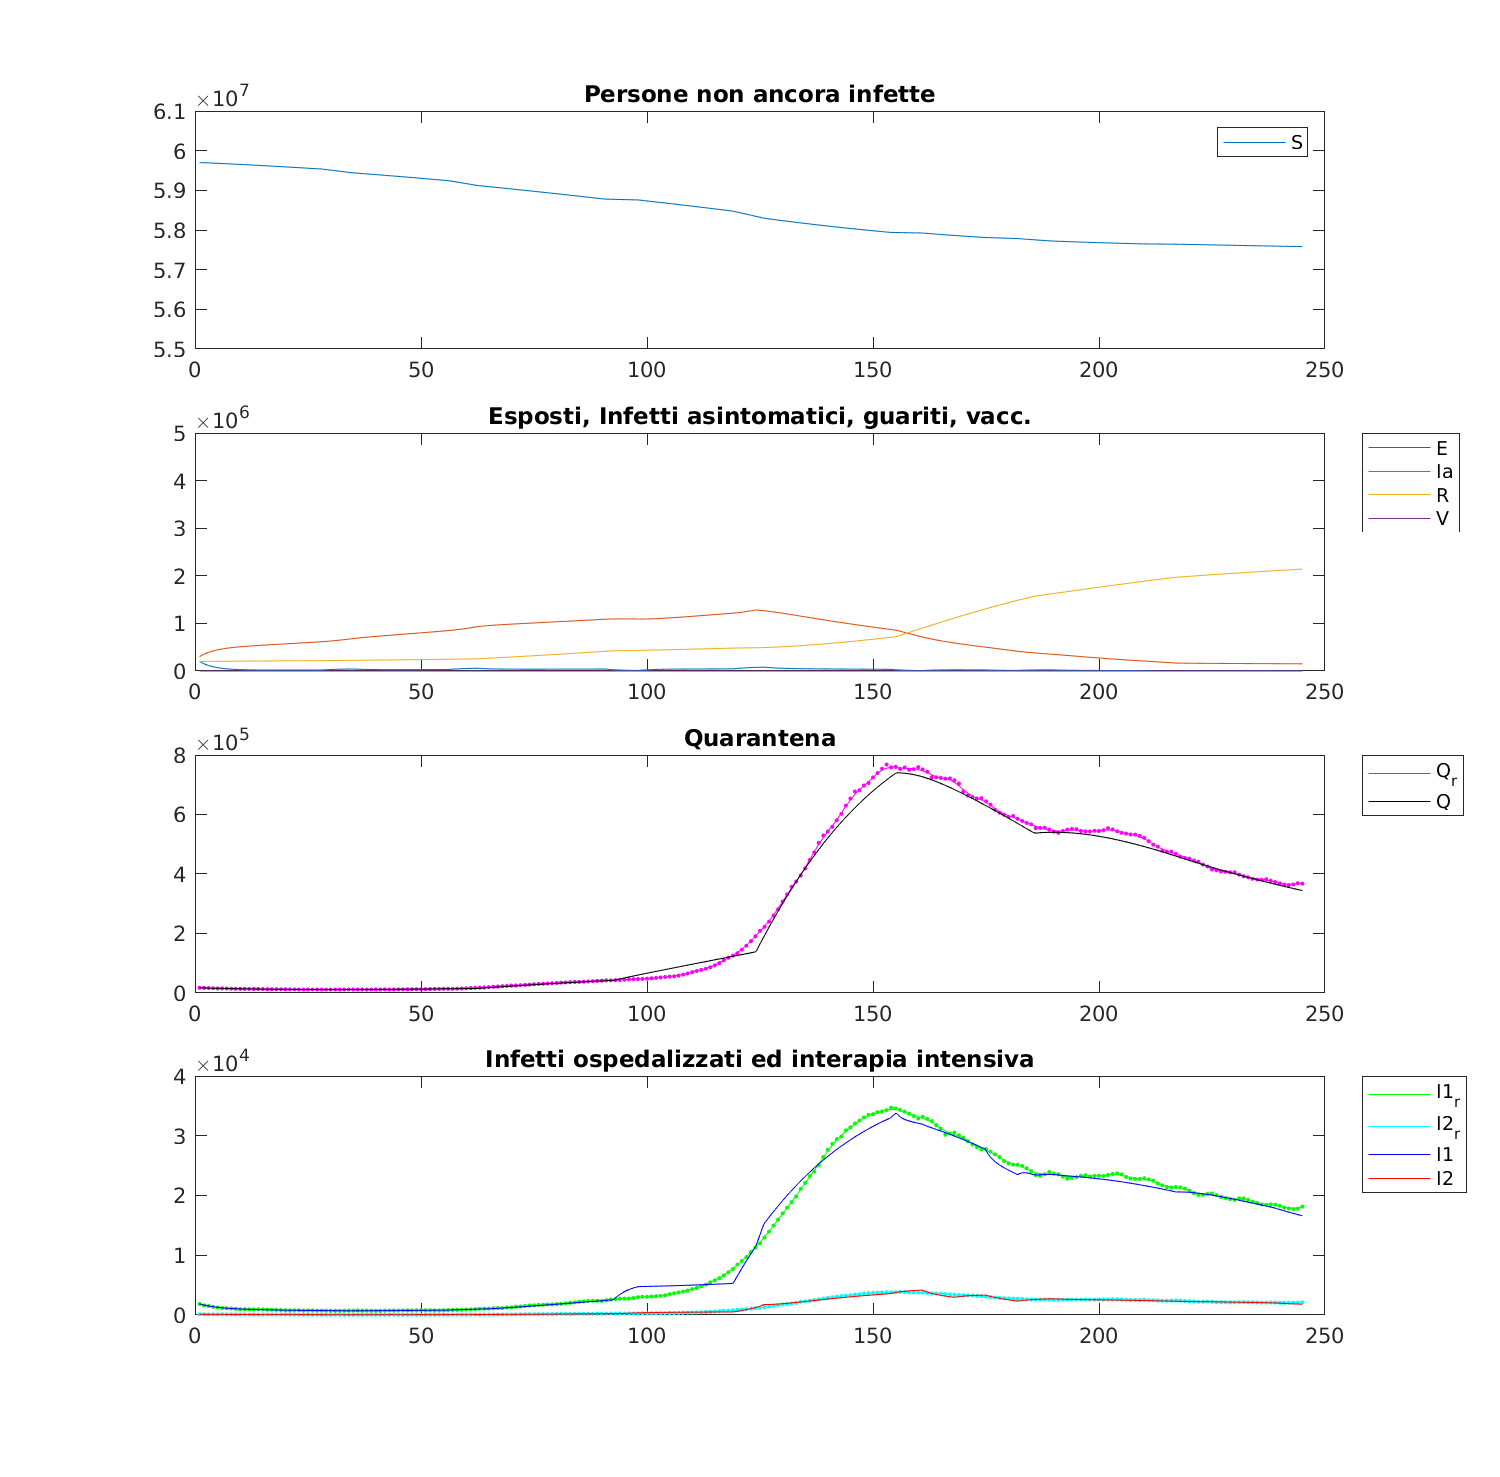
\includegraphics[width=15.215cm,height=14.995cm]{Optimalcontrolstrategies-img/Optimalcontrolstrategies-img001.png}
\end{figure}

\bigskip


\bigskip

Necessario controllo ottimo per minimizzare il carico del controllo usato minimizzando allo stesso tempo il numero di
persone infette. Infatti, un problema che tuttora è presente è la difficoltà di gestire i pazienti ospedalizzati (fare
un controllo ottimo su infetti in terapia intensiva e non, quindi I1 e I2 e allo stesso tempo minimizzare il controllo
sulle cure) 

\begin{itemize}
\item Chiedere alla professoressa il significato dei pesi imposti sul controllo delle cure (teoricamente il peso aumenta
se aumenta la conoscenza della malattia, ossia si sa come trattarla 
\end{itemize}

\bigskip


\bigskip


\bigskip


\bigskip


\bigskip


\bigskip


\bigskip


\bigskip


\bigskip


\bigskip


\bigskip

\textbf{4. Conclusions}


\bigskip


\bigskip

\section{Bibliografia}
\hypertarget{Toc66707031}{}
\bigskip

[6] https://github.com/pcm-dpc/COVID-19/blob/master/dati-andamento-nazionale/dpc-covid19-ita-andamento-nazionale.csv
\end{document}
